\section{Remote Client}
\label{sec:test-rc}

In the Remote Client application, there were many test cases to implement in order to verify all the integrity of the app.
There are two main types that can be distinguished: layout tests and logic tests.

\subsection{Layout}
\label{subsec:layout-test-rc}

On the layout tests, the main tests were functional, such as try to navigate between windows, verify some critical decisions of the user, prevent some bugs on some button click, and so on.

On fig~\ref{fig:rc-quit-test} shows the behaviour of the application when the user clicks on the exit button, while on fig~\ref{fig:rc-logout-test} shows the behave to a user trying to log out. These are just some examples of test cases on the layout that turned out to behave as expected, such as the others not mentioned.

\begin{figure}[htb!]
  \centering
  \begin{subfigure}{.45\textwidth}
    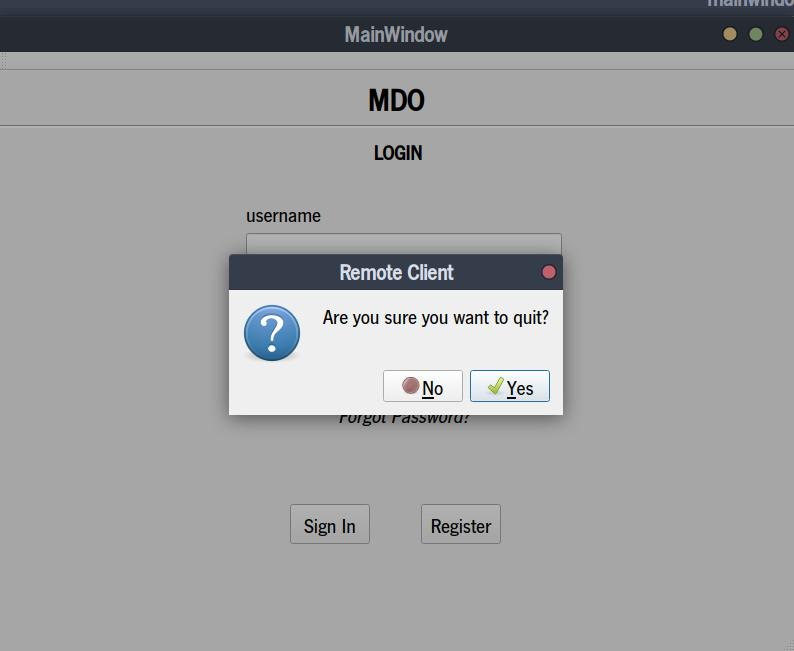
\includegraphics[width=\textwidth]{img/rc-quit-test.jpg}%
  \caption{User try to quit Test Case}%
  \label{fig:rc-quit-test}
  \end{subfigure}
  % 
  \begin{subfigure}{.45\textwidth}
    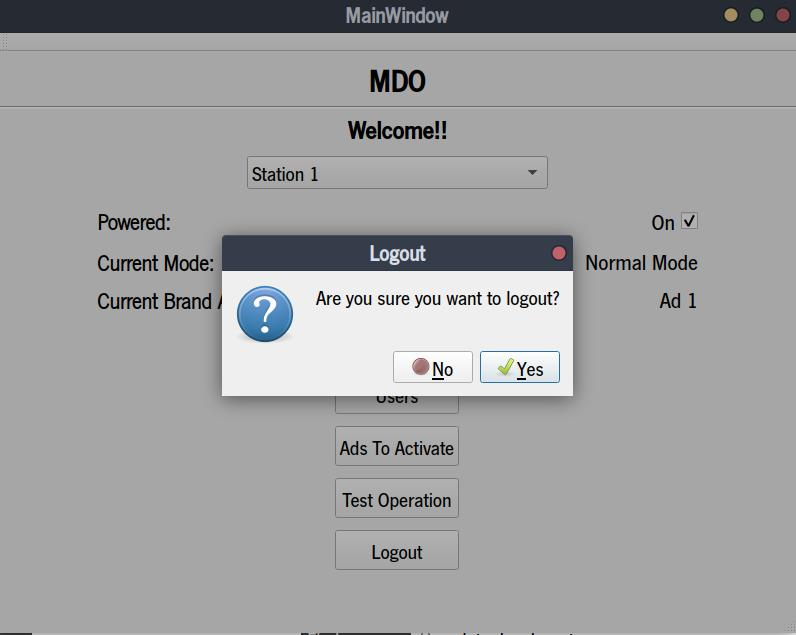
\includegraphics[width=\textwidth]{img/rc-logout-test.jpg}%
  \caption{User try to logout Test Case}%
  \label{fig:rc-logout-test}
  \end{subfigure}
  % 
  \caption{\gls{mdo-l} Layout Test Cases}%
  \label{fig:rc-layout-test}
\end{figure}

\subsection{Logic}
\label{subsec:logic-test-rc}

On the logic tests, there were two different types of tests: the ones who were only with Qt based inputs and classes and error handling with queries on MySQL Server.

\subsubsection{Interface based tests}
The interface based tests are related to validate some kind of inputs before the data processing or data sent, in order to minimize errors or unexpected scenarios as much as possible. Two examples of this type of tests can be shown on the register view, where the user needs to input a valid email with the character '@' and the string ".com" (Fig.~\ref{fig:rc-email-test}) and the need to validate the password (Fig.~\ref{fig:rc-password-test}).
%
\begin{figure}[htb!]
  \centering
  \begin{subfigure}{.45\textwidth}
    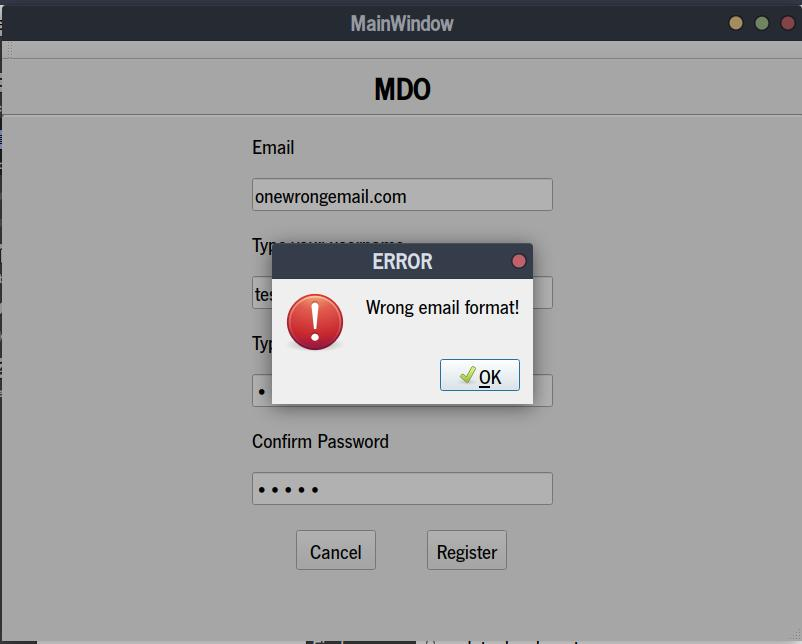
\includegraphics[width=\textwidth]{img/rc-email-test.jpg}%
  \caption{Email Register Test Case}%
  \label{fig:rc-email-test}
  \end{subfigure}
  % 
  \begin{subfigure}{.45\textwidth}
    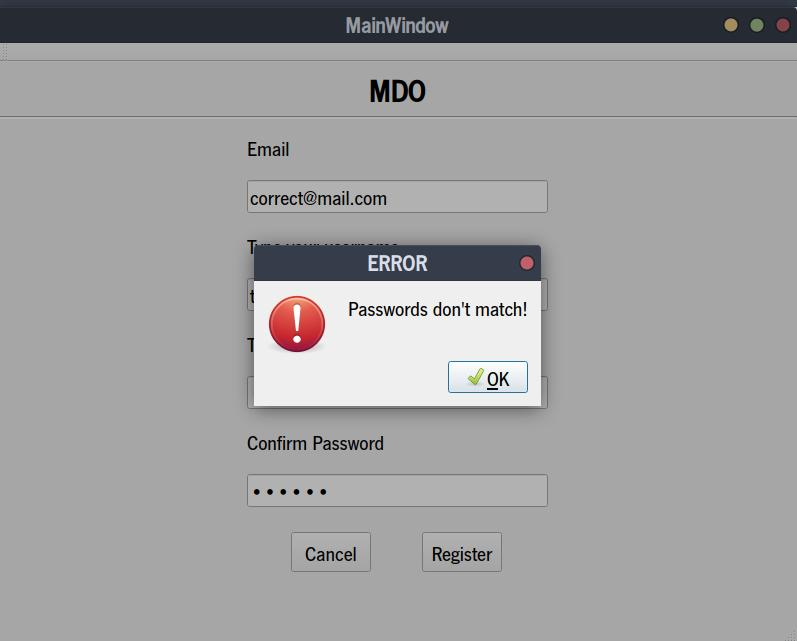
\includegraphics[width=\textwidth]{img/rc-password-test.jpg}%
  \caption{Confirm Password on Register Test Case}%
  \label{fig:rc-password-test}
  \end{subfigure}
  % 
  \caption{\gls{mdo-l} Logic (interface based) Test Cases}%
  \label{fig:rc-interface-test}
\end{figure}

\subsubsection{Error handling tests (MySQL)}
The error handling tests are related mainly with queries with MySQL that can not return as expected. One good example of that is on the login menu, because if there's no username and password matching the input, the SQL server will not return any type of data, and in this case it is necessary to handle that error and process it in the best way possible.

Fig.~\ref{fig:rc-login-test} depicts the example described above.
%
\begin{figure}[!htb]
    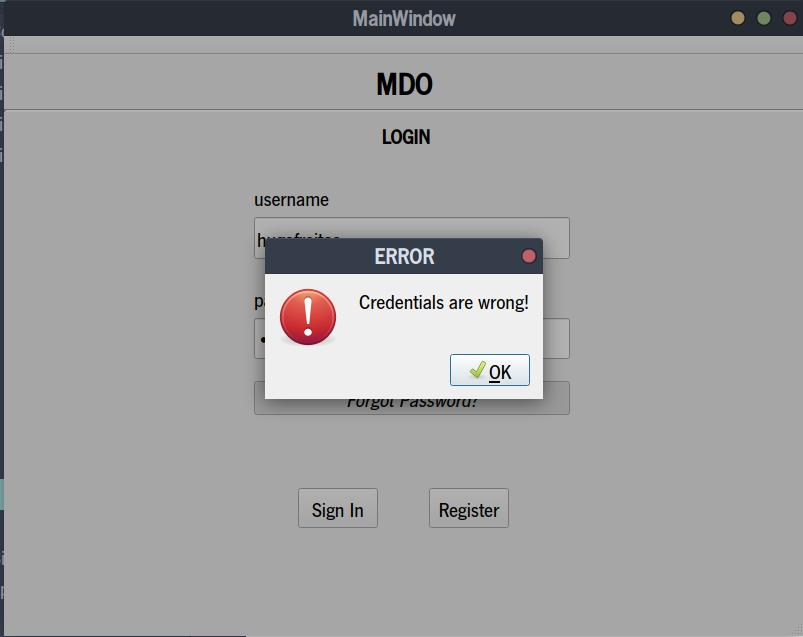
\includegraphics[width=.5\textwidth]{img/rc-login-test.jpg}%
  \caption{Bad Login Test Case}%
  \label{fig:rc-login-test}
\end{figure}

Also, tests related to ad a new user can be made to verify if a user is created. Fig~\ref{fig:rc-new-register-test} shows an example of that
%
\begin{figure}[htb!]
  \centering
  \begin{subfigure}{.45\textwidth}
    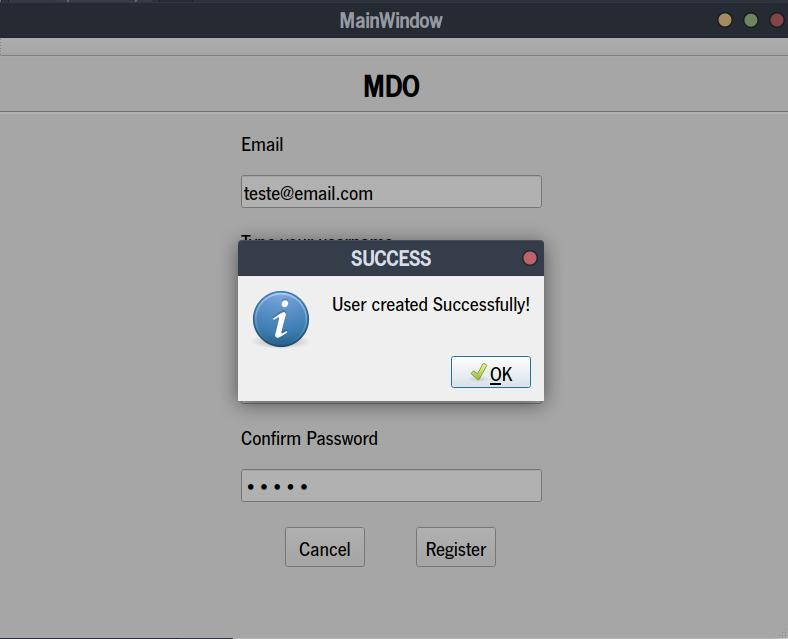
\includegraphics[width=\textwidth]{img/rc-new-register-test.jpg}%
  \caption{New Register Test Case}%
  \label{fig:rc-email-test}
  \end{subfigure}
  % 
  \begin{subfigure}{.45\textwidth}
    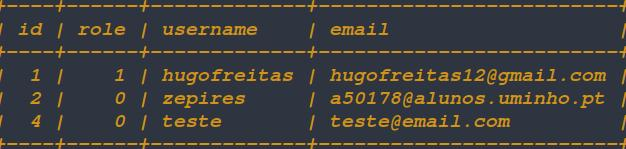
\includegraphics[width=\textwidth]{img/rc-new-register-sql-test.jpg}%
  \caption{Confirm Register on SQL Test}%
  \label{fig:rc-password-test}
  \end{subfigure}
  % 
  \caption{Register Test Case}%
  \label{fig:rc-new-register-test}
\end{figure}
%%% Local Variables:
%%% mode: latex
%%% TeX-master: "../../../dissertation"
%%% End:
